\documentclass[11pt]{article}
\usepackage[margin=0.78in]{geometry}
\usepackage{times}
\usepackage{microtype}
\usepackage{setspace}
\usepackage{booktabs}
\usepackage{tabularx}
\usepackage{array}
\usepackage{tikz}
\usetikzlibrary{positioning,arrows.meta}
\usepackage{hyperref}
\usepackage{enumitem}
\usepackage{xcolor}
\setlist{nosep,leftmargin=*}
\setstretch{1.06}
\emergencystretch=2em
\newcommand{\code}[1]{\texttt{\small #1}}
\title{VietProfs: Building a Self-Maintaining Directory of the Vietnamese Academic Diaspora}
\author{Anonymous authors for review}
\date{August 2026}

\begin{document}
\maketitle

\begin{abstract}
Public directories of specialized populations are deceptively difficult to keep accurate. The
records describe people and institutions on the open web, where appointments, titles, affiliations,
and pages change without a shared update protocol. We present VietProfs, a deployed static web
directory of Vietnamese and Vietnamese-diaspora faculty at universities outside Vietnam, as an
experience report on this problem. Its workflow combines bounded search tasks, agent-assisted
candidate generation and revalidation, structured proposals, deterministic validation, a tracked
verification ledger, and human or independent review for ambiguous cases. The central design rule
is operational rather than aspirational: AI proposes; evidence decides. As of 29 August 2026, the
canonical snapshot contains 831 records at 367 universities in 19 countries, organized into 17
broad fields and five appointment tracks. Runtime aggregation exposes institutional and disciplinary
patterns, while Git history records additions, promotions or track corrections, moves, removals, and
deduplication. We distinguish expansion---finding people not yet represented---from revalidation---
checking existing claims against the changing web. The system is not a complete census and does not
provide controlled accuracy or cost estimates. Its contribution is a concrete engineering pattern:
a public directory is a continuously revalidated collection of claims about an external world, not
merely a database snapshot.
\end{abstract}

\section{Introduction}
Structured public datasets become stale for a simple reason: the world they describe changes while
the dataset waits for an update. A faculty member is promoted, changes universities, becomes
emeritus, leaves academia, or acquires a new official profile. A URL may disappear during a site
redesign. A newly eligible person may never appear in the search results that originally seeded a
directory. Each row is consequently a claim about an external entity, and maintenance is a
reconciliation problem between those claims and a distributed, changing web.

VietProfs is a public directory of Vietnamese and Vietnamese-diaspora professors at universities
worldwide. The site is intentionally small in data-engineering terms---a static Vite application
whose canonical roster is JSON---but the population it represents is open-world, heterogeneous, and
not available from a single authoritative source. Ordinary search is insufficient because faculty
pages are inconsistently indexed, academic titles vary by country, and a plausible name or research
mention is not proof of a current appointment. Manual curation alone is difficult to sustain as the
directory grows.

This paper uses VietProfs as a case study for a broader question: how can AI-assisted automation
continuously discover, verify, correct, analyze, and maintain a public directory while retaining
evidence and human oversight? We make four bounded contributions. First, we document the data model
and operational architecture of a live directory. Second, we describe a workflow that separates
candidate discovery from evidence-backed verification. Third, we characterize expansion and
revalidation using implementation artifacts and public Git history. Fourth, we show how a maintained
roster supports reproducible descriptive observations while also creating a second maintenance
problem for derived knowledge.

\section{VietProfs and the Data Model}
\label{sec:model}
The public source of truth is \code{public/data.json}; the browser loads it and performs search,
filtering, sorting, and aggregation. A record contains a name, current profile URL, university,
city, state or province when applicable, country, department, research areas, rank and appointment
track, optional education and honors, optional Scholar and personal-site URLs, portrait provenance,
and \code{lastUpdatedAt}. The separate \code{maintenance/verification.json} ledger records the time
of a completed full review and is not part of the public site payload.

The inclusion rule is a classification policy. A person must have a current primary university
appointment outside Vietnam, except for qualifying emeritus appointments, and must fit one of five
tracks: Tenure-line, Teaching, Research, Clinical, or Emeritus. Adjunct, visiting, postdoctoral,
affiliate/courtesy, temporary, part-time, non-university, and industry-only positions are excluded.
Teaching includes stable full-time non-tenure-track appointments such as Professor of Practice;
Research and Clinical require evidence that the appointment is faculty-level and stable; Emeritus
requires a formally conferred title following a tenure-line career. The published rank is normalized
for the public vocabulary where appropriate, while institution-specific titles are preserved when
they clarify a non-tenure appointment. [CODE: \code{ROSTER\_MAINTENANCE.md}; \code{src/data.ts}]

Vietnamese identity is not inferred from a surname. Vietnamese names and common surnames are used as
search signals, but eligibility depends on the appointment and the project's inclusion policy. This
distinction matters for both ethics and correctness: \code{Nguyen} is neither sufficient evidence of
identity nor a reliable duplicate key. Names are deduplicated by person, with a university suffix
used only when genuinely identical names require disambiguation.

Departments are mapped to 17 broad fields by ordered rules and institution-specific overrides.
Health Sciences additionally has derived subfields such as Clinical Medicine, Public Health,
Nursing, Pharmacy, Dentistry, and Biomedical Research. The mapper is deliberately explicit because
strings such as ``Information Studies'' or ``Mathematics and Statistics'' can mean different things
in different institutional contexts. The tests assert both the taxonomy and representative
overrides. [CODE: src/data.ts; test/data.test.ts]

\section{Why Maintaining the Directory Is Hard}
The task has five coupled sources of uncertainty. First, it is open-world: the set of eligible
people is not enumerated anywhere, so absence from a search result is weak negative evidence.
Second, official sources are heterogeneous. A department directory, a university news article, a
CV, a personal homepage, and a conference biography have different roles and freshness. Third,
academic titles are not globally interchangeable; a research assistant professor can be a career
research rank at one institution and a temporary postdoctoral-like role at another. Fourth, identity
resolution is hard when names are common, transliterated, reordered, accented, abbreviated, or
shared by multiple people. Finally, web pages are mutable: a 404 may indicate a moved page or site
redesign rather than a departure.

These conditions make a row better understood as a claim such as ``person $p$ currently holds
appointment $a$ at institution $u$, supported by source $s$,'' with a future revalidation obligation.
The database is a materialized view of claims; the sources and review history are what make the
view maintainable.

\section{System Architecture}
Figure~\ref{fig:arch} summarizes the implemented flow. Public web sources feed either bounded
discovery or a targeted revalidation task. An agent returns a structured proposal and report. The
controller applies deterministic schema and scope checks before changing the canonical roster. The
static site is built from the resulting snapshot, while the same snapshot is later selected for
revalidation using the ledger.

\begin{figure}[t]
\centering
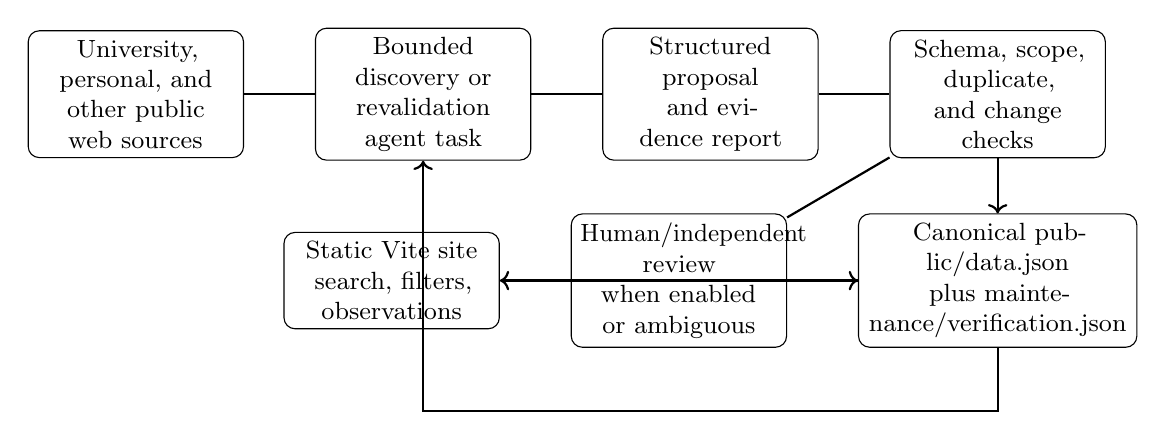
\begin{tikzpicture}[node distance=7mm and 9mm, every node/.style={font=\small}, box/.style={draw, rounded corners, align=center, minimum height=8mm, text width=25mm}, wide/.style={draw, rounded corners, align=center, minimum height=8mm, text width=33mm}, arr/.style={->, thick}]
\node[box] (web) {University, personal, and other public web sources};
\node[box, right=of web] (agent) {Bounded discovery or revalidation\\agent task};
\node[box, right=of agent] (proposal) {Structured proposal\\and evidence report};
\node[box, right=of proposal] (gate) {Schema, scope, duplicate,\\and change checks};
\node[wide, below=of gate] (canonical) {Canonical public/data.json\\plus maintenance/verification.json};
\node[box, left=of canonical] (human) {Human/independent review\\when enabled or ambiguous};
\node[box, left=of human] (site) {Static Vite site\\search, filters, observations};
\draw[arr] (web)--(agent)--(proposal)--(gate)--(canonical);
\draw[arr] (gate)--(human)--(canonical);
\draw[arr] (canonical)--(site);
\draw[arr] (canonical.south) |- ++(0,-8mm) -| (agent.south);
\end{tikzpicture}

\caption{VietProfs architecture. Solid arrows denote implemented data flow; the lower loop represents periodic revalidation.}
\label{fig:arch}
\end{figure}

\subsection{Controller and proposal boundary}
\code{scripts/maintain-roster.ts} is the unattended maintenance controller. It normally selects
entries missing from the ledger or whose last full review is at least 365 days old, prioritizing
older and incomplete records, and processes at most 40 per new run. It supports dry runs, full or
capped sweeps, name/field targeting, resumable checkpoints, safe stop/status, retry handling, and
Claude as the default research agent. Codex can be selected as the agent or enabled as an
independent review pass.

Agents cannot edit repository files directly. They return schemas for target matching, research,
and optional independent review. The controller validates required fields, HTTP(S) roles, accepted
tracks, research areas, honors and degree shapes, portrait paths, and other invariants. It also
checks that a proposal changes only the targeted record, does not reorder the roster, and does not
silently modify unrelated entries. A changed public record receives a new \code{lastUpdatedAt}; a
complete review that finds no substantive change advances only the ledger timestamp. [CODE:
scripts/maintain-roster.ts; test/maintenance-controller.test.ts]

The deployment workflow runs tests and a production build on every push to \code{main}, then deploys
the static artifact to GitHub Pages. The maintenance controller can commit and push after checks.
This is a strong degree of operational automation, but it is not a formal correctness guarantee and
does not eliminate human judgment for ambiguous evidence.

\section{Discovery as Partitioned Open-World Search}
An instruction such as ``find all Vietnamese professors at universities worldwide'' has unbounded
scope and unmeasurable recall. VietProfs instead generates repeatable queries for a bounded
university, field, and domain, combining site-restricted searches, department/faculty terms,
institutional news and research-center queries, and Vietnamese-name signals. The agent is expected
to audit existing entries, gather evidence per candidate, and treat coauthors, student pages, grants,
and research mentions as leads rather than proof. [CODE: \code{scripts/faculty-discovery-queries.ts};
DOC: \code{ROSTER\_MAINTENANCE.md}]

This decomposition is a practical form of bounded open-world search. It improves auditability: a
research pass can say which university/field/country slice it attempted, what was added, and in
some cases that no eligible addition was found. It does not solve recall. Search-engine ranking,
English-language visibility, uneven university websites, and differing effort across slices remain
sampling mechanisms. The repository history shows a switch to country-by-country searches, batches
for international universities, and field audits. These are operational strategies, not evidence
of exhaustive coverage.

\section{Evidence and Verification}
\label{sec:evidence}
Discovery is not verification. A candidate enters the workflow because a query or lead suggests a
person; publication requires evidence that the person is current, at the claimed institution and
department, in an eligible track, with a working official profile. Official faculty pages are the
preferred source. Personal pages and CVs can supply details, but the current appointment is still
confirmed on an official source where possible. Search snippets, conference biographies, and
coauthorship are leads or corroboration rather than default authority.

The implementation therefore follows the rule ``AI proposes; evidence decides.'' The agent can
read public pages, compare an old record with current evidence, and produce structured data, but the
controller does not treat free-form model text as canonical state. The proposal schema requires an
action, status, report, sources, and proposed JSON; an optional independent Codex review can approve,
reject, or mark uncertain. Rejected proposals receive bounded revisions in the configured workflow;
incomplete or uncertain work is deferred rather than marked successfully verified.

The evidence model is practical rather than a formal confidence score. URLs are retained for the
profile, honors, portrait, and optional personal/Scholar pages, and Git preserves the resulting
patch. There is no per-field provenance graph or source snapshot store. This is an important
limitation: a URL is evidence access, not a cryptographic proof that the page had a particular
content at review time.

\section{Continuous Revalidation and Self-Maintenance}
\label{sec:maintenance}
VietProfs separates two loops, shown in Figure~\ref{fig:lifecycle}. Expansion starts from an
unsearched slice and tries to add a new verified record. Revalidation starts from an existing record
and checks whether its claim still matches the web. The latter checks profile liveness and role,
URL-role correctness, Scholar identity, current rank/track, education, honors, and possible moves;
it also looks for new candidates incidentally. The ledger allows the controller to choose the least
recently reviewed records rather than repeatedly touching only newly added people.

\begin{figure}[t]
\centering
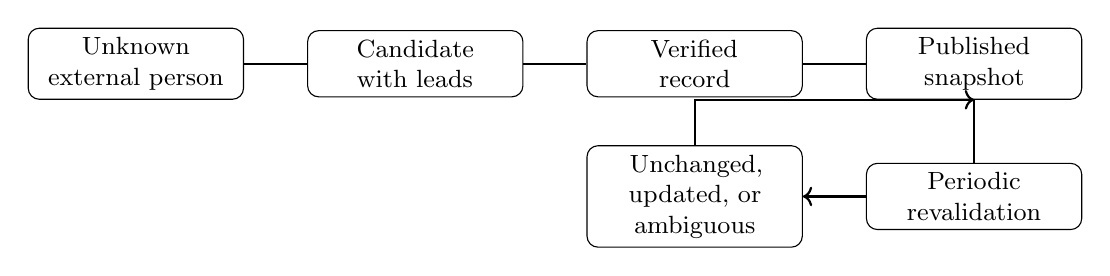
\begin{tikzpicture}[node distance=8mm and 8mm, every node/.style={font=\small}, box/.style={draw, rounded corners, align=center, minimum height=8mm, text width=25mm}, arr/.style={->, thick}]
\node[box] (unknown) {Unknown\\external person};
\node[box, right=of unknown] (candidate) {Candidate\\with leads};
\node[box, right=of candidate] (verified) {Verified\\record};
\node[box, right=of verified] (published) {Published\\snapshot};
\node[box, below=of published] (recheck) {Periodic\\revalidation};
\node[box, left=of recheck] (changed) {Unchanged,\\updated, or ambiguous};
\draw[arr] (unknown)--(candidate)--(verified)--(published)--(recheck)--(changed);
\draw[arr] (changed.north) |- (published.south);
\end{tikzpicture}

\caption{Record lifecycle. A published record is not terminal; it returns to the revalidation loop.}
\label{fig:lifecycle}
\end{figure}

Negative evidence requires caution. A disappeared faculty page can mean redesign, a moved URL,
temporary failure, a university move, retirement, or departure. The maintenance policy explicitly
avoids treating \code{404} as automatic deletion and calls for corroboration. Removal is also a
stronger action than addition because it destroys a public claim and can erase a legitimate person
from the directory. The system supports removal proposals, but the guide's corroboration rule is an
operational policy rather than a formally verified deletion protocol.

The Git history makes this lifecycle visible. A 20-batch full-roster refresh appears on 26 August
2026. Subsequent history records automated maintenance batches, country sweeps, a Teaching-to-
Clinical correction, a duplicate merge, a university-name canonicalization, a corrected affiliation,
and a policy-based removal. These examples show that maintenance is not a periodic cosmetic edit;
it changes eligibility, identity, affiliation, and derived data assumptions.

\section{What the Directory Reveals}
\label{sec:results}
The site has a third function beyond building and maintaining knowledge: learning from the current
roster. Primary knowledge is the individual record. Aggregation produces derived knowledge such as
institutional concentration, field balance, geography, track distribution, awards, and doctoral
institution patterns.

\subsection{Runtime observations}
The ``Show me something interesting'' view is computed at runtime from the current JSON snapshot.
It reports U.S. and international counts, state/country groups, institution groups, same-institution
same-field clusters, field comparisons, award summaries, PhD cohorts, and leaderboards. It stores no
hand-written facts. Tests require multi-record, roster-only observations and reject unsupported
surname, prestige, demographic, causal, or population claims. The result is therefore a descriptive
view, not an estimate of the entire diaspora. [CODE: src/data.ts; src/main.ts; test/data.test.ts]

\subsection{Snapshot observations}
Table~\ref{tab:snapshot} summarizes the current snapshot. Within it, Monash University has 13
records, UC San Diego 12, and NUS 11. California and Texas contain 169 of 554 U.S. records (31\%).
The international subset contains 277 records across 18 non-U.S. country values. The four largest
broad fields in the analysis are Computer and Information Sciences (132), Engineering (124),
Business and Economics (112), and Health Sciences (99). Nanyang Technological University has six
engineering records; the University of Minnesota has six health-science records; and the University
of Technology Sydney has six engineering records. These are useful because they reveal institutional
and disciplinary structure without claiming prestige, population size, or causation.

\begin{table}[t]
\centering
\caption{Current VietProfs snapshot and evidence-field coverage.}
\label{tab:snapshot}
\small
\begin{tabular}{lr@{\qquad}lr}
\toprule
Records & 831 & Universities & 367\\
Countries & 19 & U.S./international & 554/277\\
Broad fields & 17 & Accepted tracks & 5\\
Profile URLs & 831 & Scholar URLs & 325\\
PhD institutions & 656 & PhD years & 488\\
Honors-bearing records & 178 & PhD-year range & 1962--2026\\
\bottomrule
\end{tabular}
\end{table}

\subsection{Derived knowledge also becomes stale}
If a person moves, an institutional count changes. If a track is corrected, the track distribution
changes. If a record is removed, a field comparison or same-institution cluster may no longer hold.
The current implementation recomputes the visible observations from the live roster at render time,
so the runtime view does not preserve stale fact text. It does not maintain a separate dependency
graph for persisted derived facts because those facts are not persisted. A future system that stores
notable findings would need dependencies, recomputation, and invalidation policies just as primary
records do.

\section{Operational Experience and Evaluation}
This work is an operational characterization, not a controlled experiment. The repository provides
strong evidence about implementation and history but not precision, recall, cost, or detection
latency. The current snapshot has 701 Tenure-line, 68 Teaching, 37 Emeritus, 21 Clinical, and 4
Research records. It contains 103 personal/lab URLs, 325 Scholar URLs, and 178 records with at least
one honor. These figures describe fields present in the snapshot, not their correctness or
completeness.

\begin{table}[t]
\centering
\caption{Representative public maintenance events in Git history.}
\label{tab:cases}
\small
\begin{tabularx}{\linewidth}{@{}p{0.18\linewidth}p{0.27\linewidth}X@{}}
\toprule
Case & Repository evidence & Result\\
\midrule
Duplicate & \code{2aa15c0}; University of Dayton & Duplicate entries for Tam V. Nguyen merged.\\
Policy removal & \code{9a4a171}; inclusion-standard decision & Nhung Nguyen (UCSF) removed.\\
Track correction & \code{ba71beb}; BU Dental & Teaching changed to Clinical.\\
Affiliation correction & \code{c1f4380} & Nguyen-Truc-Dao Nguyen affiliation corrected.\\
Name/identity cleanup & \code{c0c0603}, \code{4212955} & True duplicate, suffix, and university-name canonicalization fixed.\\
\bottomrule
\end{tabularx}
\end{table}

The event history nevertheless supports meaningful engineering observations. Batch commits make
large work reviewable; checkpoints make long agent sessions resumable; tests encode invariants such
as unique names, unique profiles, valid tracks, and targeted proposal scope; and the ledger separates
``reviewed'' from ``changed.'' The absence of candidate-level telemetry is equally important. There
is currently no denominator for candidates considered, no rejection taxonomy, no measured human
review rate, and no time-to-detection metric.

\section{What Does Not Work}
Unbounded LLM enumeration is a poor source of a canonical roster. It omits people, hallucinates
affiliations, and cannot provide a defensible stopping condition. Surname inference is unsafe and
ethically inadequate. Search snippets are stale and incomplete. Direct model writes would make it
difficult to constrain scope, distinguish a proposed change from an approved one, or recover from a
mistaken bulk edit. VietProfs instead requires structured proposals and targeted changes.

Other failures are subtler. A broad title such as ``Research Assistant Professor'' cannot establish
eligibility by itself. A page disappearance is not a departure. A personal homepage is not the same
source role as an official university profile. Department keywords misclassify ambiguous institutional
contexts unless overrides are maintained. Finally, a current count cannot be described as growth or
a migration path without versioned historical data and an explicit comparison. These lessons are
implemented in policy, tests, and recent corrective commits, but they remain areas for ongoing
measurement.

\section{Limitations and Ethics}
VietProfs is not a census. Coverage is affected by search effort, English-language discoverability,
university web quality, public-profile availability, initial field emphasis, international title
conventions, and the differing maturity of collection passes. The 554/277 U.S./international split
must not be interpreted as a population ratio. Nor should current concentrations be interpreted as
prestige, demographic size, causation, migration history, or research quality.

The directory handles sensitive identity-adjacent information. It should not infer ethnicity or
national origin from names, and it should publish only public professional information necessary for
the directory's purpose. Portraits, honors, and education need source and scope rules. Public
submission and correction mechanisms help people contest errors, but a future release should expose
clear removal/contact policy, retention expectations, and an audit trail for disputed changes.

\section{General Lessons}
The case study suggests the following design principles for agent-maintained public datasets:
\begin{enumerate}
\item Use language models primarily for candidate generation, comparison, and research assistance;
  do not make them the source of truth.
\item Separate discovery, evidence collection, verification, proposal, and canonical application.
\item Attach source URLs and review timestamps to claims, while recognizing that URLs alone are not
  complete provenance.
\item Partition open-world search into bounded, repeatable tasks.
\item Treat removal and negative evidence as higher-risk than addition.
\item Keep candidate state separate from canonical state and constrain proposed edits to a target.
\item Reserve human attention for ambiguity, identity resolution, policy exceptions, and disputes.
\item Design telemetry before deployment: outcomes, reasons, cost, latency, and reviewer actions.
\item Recompute or invalidate derived knowledge when primary claims change.
\end{enumerate}
Together these principles implement the operational slogan ``AI proposes; evidence decides'' without
pretending that the web or the model is fully reliable.

\section{Related Work}
VietProfs is related to entity resolution, web extraction, scholarly knowledge graphs, and
provenance-aware maintenance, but it is not a replacement for a general scholarly index. Surveys of
entity resolution emphasize end-to-end blocking, matching, and data-quality pipelines over
heterogeneous descriptions \cite{christophides2019er,elmagarmid2007duplicate}. Recent work studies
LLMs for entity matching, including prompt sensitivity, structured explanations, and robustness to
unseen entities \cite{peeters2023llm}; another line explicitly treats model queries as a costed
uncertainty-reduction resource \cite{li2024er}. VietProfs uses the practical implication---models
can help compare and organize evidence---but does not claim their reported benchmark performance
for this domain.

Knowledge-graph maintenance work formalizes incremental updates and provenance for asserted and
derived facts \cite{belhajjame2023maintenance}. VietProfs is simpler: JSON records, URLs, Git
history, and runtime aggregation rather than an RDF graph or why-provenance engine. The conceptual
connection is nevertheless direct: when a source claim changes, dependent answers may change.

OpenAlex provides a useful contrast as a large, open scholarly knowledge graph of works, authors,
venues, institutions, and concepts \cite{priem2022openalex}. VietProfs has a narrower population,
more detailed appointment eligibility, and a public-directory interaction model. DBLP and ORCID are
also important reference ecosystems for scholarly identity, but VietProfs's engineering problem is
the current faculty appointment and its evidence, not publication identity alone. The contribution
here is therefore an experience report about a specialized, continuously revalidated directory and
the operational boundary between agent assistance and canonical data.

\section{Conclusion}
Small specialized public datasets used to be expensive to maintain because every correction required
continuous human labor against a changing web. VietProfs shows how that labor can be reduced with
bounded agent tasks, structured proposals, deterministic invariants, provenance links, resumable
revalidation, and human oversight. It also shows why automation is not the same as autonomy: the
directory remains incomplete, sources conflict, titles are ambiguous, and derived knowledge can
become stale.

The broader view is that a public directory is a continuously revalidated collection of claims about
a changing external world. The useful system boundary is therefore not ``LLM writes JSON,'' but
``agents propose evidence-backed changes to a constrained claim store, which is periodically
reconciled with its sources.'' As the cost of this reconciliation falls, more specialized public
knowledge resources may become practical to sustain---provided their authors measure coverage,
retain provenance, support correction, and state clearly what the data does and does not establish.

\bibliographystyle{plain}
\bibliography{references}
\end{document}
